\tikzstyle{empty}   = [pin edge={to-,thin,black}]
\tikzstyle{circ}    = [circle, minimum size=1cm, text centered, draw=black, fill=blue!20]
\tikzstyle{arrow} = [very thin,->,>=stealth]
\tikzstyle{thick_arrow} = [thick,->,>=stealth]

\tikzstyle{reg_perc}  = [circle, fill=blue!20]
\tikzstyle{conv_perc} = [circle, fill=red!20]
\tikzstyle{output} =    [circle, fill=green!20]


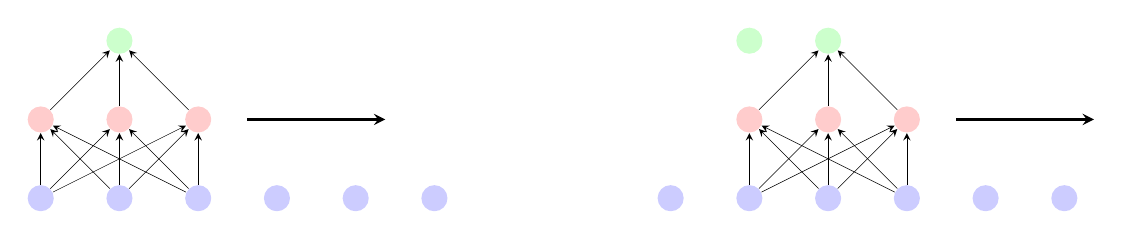
\begin{tikzpicture}
    %%%% PRODUCING FIRST OUTPUT %%%% 
    % Conv filter
    \node (cperc0) [conv_perc] {};
    \node (cperc1) [conv_perc, right of=cperc0] {};
    \node (cperc2) [conv_perc, right of=cperc1] {};
    % Empty nodes for arrow showing filter movement
    \node (empty_node1) [empty, right of=cperc2, xshift=-0.5cm] {};
    \node (empty_node2) [empty, right of=empty_node1, xshift=1cm] {};
    % Layer below conv
    \node (perc0) [reg_perc, below of=cperc0] {};
    \node (perc1) [reg_perc, below of=cperc1] {};
    \node (perc2) [reg_perc, below of=cperc2] {};
    \node (perc3) [reg_perc, right of=perc2] {};
    \node (perc4) [reg_perc, right of=perc3] {};
    \node (perc5) [reg_perc, right of=perc4] {};
    % Output of conv filter
    \node (output) [output, above of=cperc1] {};
    %% Arrows
    % conv_perc0
    \draw [arrow] (perc0) -- (cperc0);
    \draw [arrow] (perc1) -- (cperc0);
    \draw [arrow] (perc2) -- (cperc0);
    % conv_perc1
    \draw [arrow] (perc0) -- (cperc1);
    \draw [arrow] (perc1) -- (cperc1);
    \draw [arrow] (perc2) -- (cperc1);
    % conv_perc2
    \draw [arrow] (perc0) -- (cperc2);
    \draw [arrow] (perc1) -- (cperc2);
    \draw [arrow] (perc2) -- (cperc2);
    % Output
    \draw [arrow] (cperc0) -- (output);
    \draw [arrow] (cperc1) -- (output);
    \draw [arrow] (cperc2) -- (output);
    % Arrow for illustrating filter movement
    \draw [thick_arrow] (empty_node1) -- (empty_node2);
    
    %%%% PRODUCING SECOND OUTPUT %%%%
    % Layer below conv
    \node (perc10) [reg_perc, right of=perc5, xshift=2cm] {};
    \node (perc11) [reg_perc, right of=perc10] {};
    \node (perc12) [reg_perc, right of=perc11] {};
    \node (perc13) [reg_perc, right of=perc12] {};
    \node (perc14) [reg_perc, right of=perc13] {};
    \node (perc15) [reg_perc, right of=perc14] {};
    % Conv filter
    \node (cperc10) [conv_perc, above of=perc11] {};
    \node (cperc11) [conv_perc, above of=perc12] {};
    \node (cperc12) [conv_perc, above of=perc13] {};
    % Output
    \node (output11) [output, above of=cperc11] {};
    \node (output10) [output, left of=output11] {};
    % Empty nodes for arrow showing filter movement
    \node (empty_node11) [empty, right of=cperc12, xshift=-0.5cm] {};
    \node (empty_node12) [empty, right of=empty_node11, xshift=1cm] {};
    %% Arrows
    % conv_perc0
    \draw [arrow] (perc11) -- (cperc10);
    \draw [arrow] (perc12) -- (cperc10);
    \draw [arrow] (perc13) -- (cperc10);
    % conv_perc1
    \draw [arrow] (perc11) -- (cperc11);
    \draw [arrow] (perc12) -- (cperc11);
    \draw [arrow] (perc13) -- (cperc11);
    % conv_perc2
    \draw [arrow] (perc11) -- (cperc12);
    \draw [arrow] (perc12) -- (cperc12);
    \draw [arrow] (perc13) -- (cperc12);
    % Output
    \draw [arrow] (cperc10) -- (output11);
    \draw [arrow] (cperc11) -- (output11);
    \draw [arrow] (cperc12) -- (output11);
    % Arrow for illustrating filter movement
    \draw [thick_arrow] (empty_node11) -- (empty_node12);
\end{tikzpicture}